\section{Force estimation at known positions}\label{sec:forces}
\subsection{Estimator and residual-based weights}
The 31 fitted acceleration channels estimate forces at the known positions
and directions in $B$; measured interface forces serve as the reference.
After mean removal, a real DFT of each 60 s record gives $1/60$ Hz spacing.
Only the 38401 lines in 360--1000 Hz are retained. At each line, write
\[
 a=H_\theta f+e,\qquad H_w=D^{-1}H_\theta,\qquad
 D=\diag(d_1,\ldots,d_m),\quad d_o>0.
\]
For $\rank H_w=p$, the weighted least-squares estimate is unique:
\begin{equation}
 f_\theta=H_w^\dagger D^{-1}a
 =\bigl(H_\theta^*D^{-2}H_\theta\bigr)^{-1}H_\theta^*D^{-2}a.
 \label{eq:force-estimator}
\end{equation}
Here $\dagger$ is the Moore--Penrose inverse; $H_\theta$ uses the retained
force columns and $s=\mathrm i2\pi\nu$. The weights are built from the
training-record FRF residuals,
\[
 d_o(\nu)^2=\operatorname{Interp}_\nu\left[
 \operatorname{Average}_{\ell\text{ in window}}\,
 \frac12\sum_{i=1}^{2}|[H_\theta(s_\ell)-\widehat H_\ell]_{oi}|^2\right].
\]
Window averages use the 0.05 Hz grid and the actual number of available
samples at the band edges. The width \ForceWindow\ Hz minimizes mean
two-force relative error on monitoring record 101 among candidates
0.25--20 Hz (Table~\ref{tab:force-selection}); it is then frozen.
These are transfer-error weights, not calibrated noise variances:
Eq.~\eqref{eq:force-estimator} is the best linear unbiased estimate only if
$\mathbb E[e]=0$ and $\mathbb E[ee^*]=cD^2$ for some $c>0$, which is not
established here.

The inverse DFT gives band-limited estimates and references. Relative RMS
errors use $6\le t\le58$ s, excluding the first 6 s and last 2 s of the
record. The fixed 50 ms display starts at 20 s; displayed spectra are
one-sided Welch averages \citep{welch1967} over the same interval with 1 s
Hann windows and 50\% overlap. For window weights $w_t$ and sample rate
$\nu_{\rm s}=8192$ Hz, each segment is normalized by
$2/(\nu_{\rm s}\sum_tw_t^{2})$, without the factor two at DC or Nyquist. No gain, delay or inverse regularization is fitted. Regularized alternatives include Tikhonov and
truncated-SVD methods
\citep{tikhonov1977,hansen1992,hansen1998,jacquelin2003,thite2003,sanchez2014};
time-domain alternatives augment the state with unknown forces
\citep{lourens2012,lourens2012b,maes2015}.

\begin{table}[tb]\centering
\begin{tabular}{llrr}\toprule
Weighting & Window [Hz] & P6 error [\%] & P8 error [\%]\\\midrule
signal level & -- & 24.7 & 11.2\\
training error spectrum & 0.25 & 18.0 & 6.8\\
training error spectrum (selected) & 0.5 & 17.8 & 6.7\\
training error spectrum & 1 & 17.8 & 6.7\\
training error spectrum & 2 & 18.2 & 6.7\\
training error spectrum & 5 & 19.3 & 7.0\\
training error spectrum & 10 & 20.3 & 7.4\\
training error spectrum & 20 & 21.3 & 8.0\\
\bottomrule\end{tabular}

\caption{Weight-window selection on record 101: relative RMS force errors
over 6--58 s. The signal-level baseline uses the scales of
Appendix~\ref{sec:fit-details}. Records 103 and 104 do not select the window.}
\label{tab:force-selection}
\end{table}

For the true transfer $H$ and measurement noise $n$, the exact error identity
and its sensitivity bound are
\begin{equation}
 e=(H-H_\theta)f+n,\qquad
 f_\theta-f=H_w^\dagger D^{-1}e,\qquad
 \|f_\theta-f\|_2\le\frac{\|D^{-1}e\|_2}{\sigma_{\min}(H_w)}.
 \label{eq:force-error}
\end{equation}
Full column rank permits inversion; the smallest singular value controls
error amplification. Neither follows from the number of sensors alone.

\subsection{Two forces: record 103}
\begin{figure}[tb]\centering
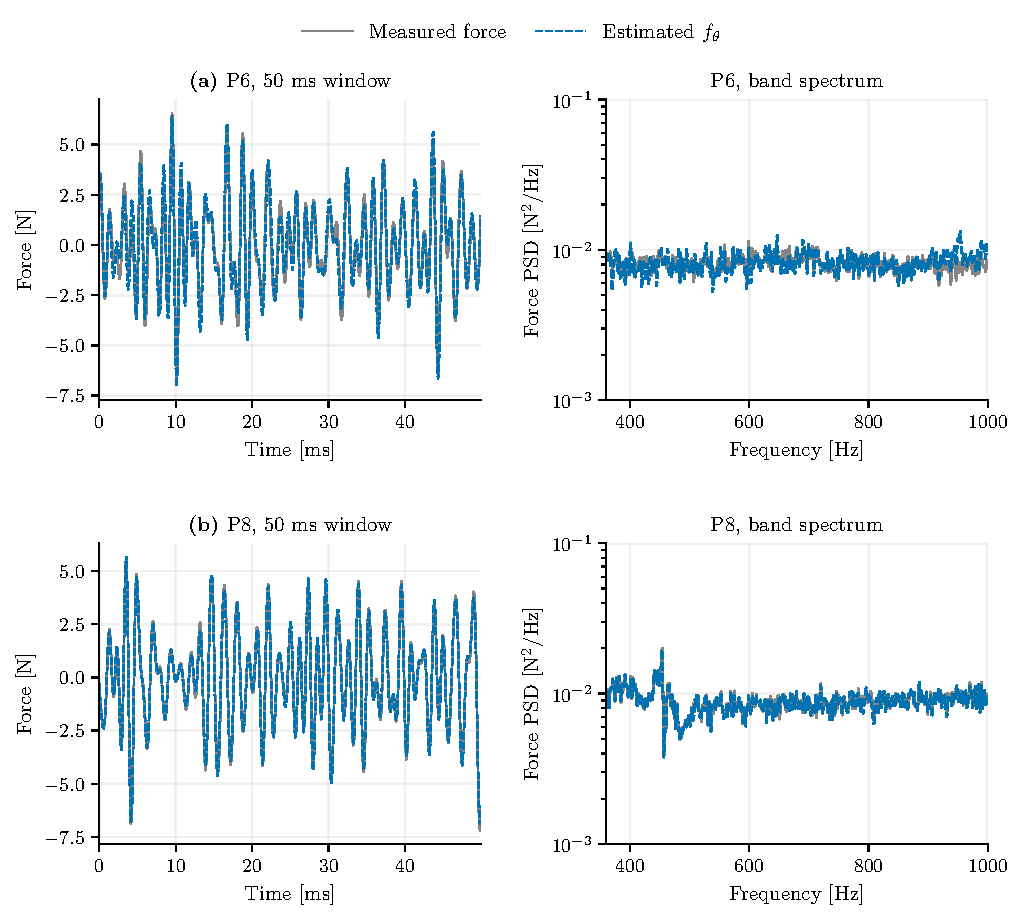
\includegraphics[width=0.95\linewidth]{force_two.pdf}
\caption{Two-force estimates on record 103 from 31 accelerations:
(a) P6 and (b) P8. Grey: measured; blue dashed: estimated. Left: 50 ms of
band-limited force starting at 20 s. Right: Welch autospectra over
6--58 s (1 s Hann windows, 50\% overlap).}
\label{fig:force-two}
\end{figure}
Both P6 and P8 carry random inputs, so $p=2$. The weighted transfer has
median condition number \ForceTwoCondition\ and maximum
\ForceTwoConditionMax\ over the band. Figure~\ref{fig:force-two} compares
the estimates with the measured forces; their assessment values are
\[
 \begin{array}{lcc}
 &\mathrm{P6}&\mathrm{P8}\\
 \text{measured RMS (N)}&\ForceTwoRmsSix&\ForceTwoRmsEight\\
 \text{estimated RMS (N)}&\ForceTwoEstRmsSix&\ForceTwoEstRmsEight\\
 \text{relative error (\%)}&\ForceTwoErrorSix&\ForceTwoErrorEight\\
 \text{correlation}&\ForceTwoCorrSix&\ForceTwoCorrEight\\
 \text{signal-level-weight error (\%)}&\ForceTwoLevelSix&\ForceTwoLevelEight
 \end{array}
\]
The median fraction of weighted acceleration energy explained per line is
\ForceTwoFit\%. Record 103 retains the development exposure described in
Section~\ref{sec:lab}.

\begin{figure}[tb]\centering
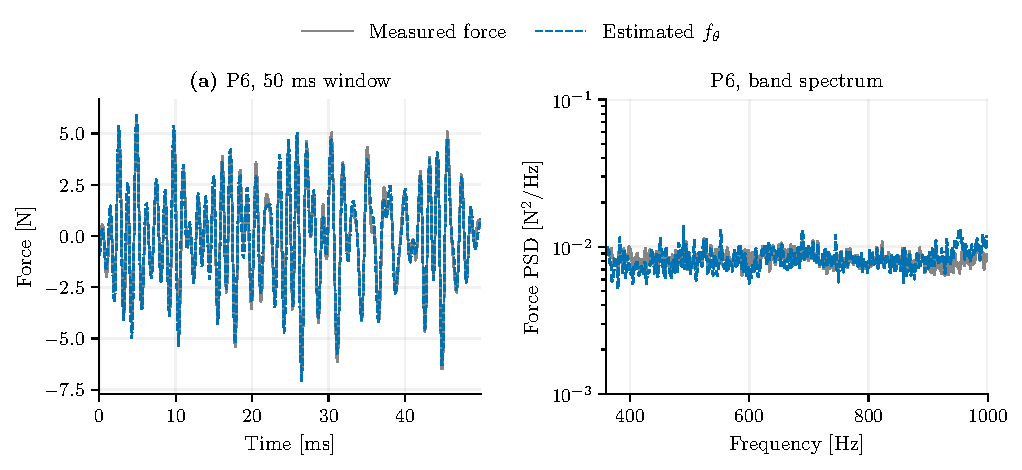
\includegraphics[width=\linewidth]{force_one.pdf}
\caption{Record 104 under the one-force approximation: P6 measured (grey)
and estimated (blue dashed), over 50 ms starting at 20 s and as Welch
autospectra over 6--58 s. The estimate uses only the P6 transfer column.}
\label{fig:force-one}
\end{figure}

\subsection{One-force approximation: record 104}
Record 104 was acquired two minutes after record 103 and was not used in
fitting, monitoring or development assessment. P6 carries a random input;
P8 carries a ramp concentrated below 100 Hz. In 360--1000 Hz, P8 retains
\ForceOneRampFraction\% of its power and has RMS \ForceOneRampRms\ N,
compared with \ForceOneRandomRms\ N for P6. The approximation $p=1$ uses
only the P6 column of $H_\theta$. Its results are
\[
 \begin{aligned}
 \text{relative error}&=\ForceOneError\%,&
 \text{correlation}&=\ForceOneCorr,\\
 \text{estimated RMS}&=\ForceOneEstRms\ \mathrm N,&
 \text{median explained energy}&=\ForceOneFit\%,\\
 \text{signal-level-weight error}&=\ForceOneLevel\%.&&
 \end{aligned}
\]
Allowing both force columns gives P6 error \ForceOneBothSix\% but assigns
\ForceOneBothEightRms\ N RMS to P8, versus \ForceOneRampRms\ N measured.
The assumed force set thus decides where model residuals go; the small
in-band P8 contribution remains in the residual of the one-force estimate.

\FloatBarrier
